\documentclass[11pt]{article}
\usepackage[margin=1in,headheight=14pt]{geometry}
\usepackage{amsmath,amssymb,amsthm,mathtools}
\usepackage[T1]{fontenc}
\usepackage{lmodern,microtype}
\usepackage{xcolor,graphicx,booktabs,tabularx,array}
\usepackage{tikz}
\usetikzlibrary{arrows.meta,positioning,calc,fit,decorations.pathreplacing}
\usepackage{enumitem,caption,needspace,fancyhdr}
\definecolor{Ink}{HTML}{15334A}
\definecolor{Blue}{HTML}{0077BB}
\definecolor{Teal}{HTML}{008577}
\definecolor{Orange}{HTML}{C65D21}
\definecolor{Mist}{HTML}{F1F6F8}
\definecolor{Rule}{HTML}{CAD8DE}
\usepackage[colorlinks=true,linkcolor=Ink,citecolor=Teal,urlcolor=Blue]{hyperref}
\hypersetup{pdftitle={A subcubic quantum Fourier transform for the symmetric group},
  pdfauthor={Nate Stemen},pdfsubject={Coherent direct induction and finite-gate complexity}}
\captionsetup{font=small,labelfont={bf,color=Ink},skip=8pt}
\setlist{itemsep=3pt,topsep=5pt}
\setlength{\emergencystretch}{3em}
\setlength{\parskip}{3pt}
\setlength{\textfloatsep}{16pt plus 3pt minus 3pt}
\setlength{\floatsep}{14pt plus 3pt minus 3pt}
\pagestyle{fancy}
\fancyhf{}
\fancyhead[L]{\small\textsc{A subcubic symmetric-group QFT}}
\fancyhead[R]{\small Nate Stemen}
\fancyfoot[C]{\small\thepage}
\renewcommand{\headrulewidth}{0.3pt}
\newtheorem{theorem}{Theorem}
\newtheorem{lemma}[theorem]{Lemma}
\newtheorem{proposition}[theorem]{Proposition}
\theoremstyle{definition}
\newtheorem{definition}[theorem]{Definition}
\newtheorem{remark}[theorem]{Remark}
\newcommand{\ket}[1]{\lvert #1\rangle}
\newcommand{\bra}[1]{\langle #1\rvert}
\newcommand{\norm}[1]{\lVert #1\rVert}
\newcommand{\F}{\mathcal F}
\newcommand{\Id}{\mathrm I}
\newcommand{\poly}{\operatorname{poly}}
\newcommand{\SYT}{\operatorname{SYT}}
\newcommand{\cont}{\operatorname{cont}}
\newcommand{\softO}{\widetilde O}
\DeclareMathOperator{\atan}{arctan}
\tikzset{
  flow/.style={-{Stealth[length=2.3mm]},draw=Ink,line width=.85pt},
  panel/.style={rounded corners=3pt,draw=Rule,fill=Mist,line width=.7pt,
    align=center,inner sep=8pt,font=\small},
  smalllabel/.style={font=\scriptsize,text=Ink,align=center},
  cell/.style={draw=Ink,line width=.65pt,minimum size=5.5mm,inner sep=0pt},
  added/.style={cell,fill=Teal!17,text=Ink,font=\bfseries},
}
\title{\color{Ink}\LARGE\bfseries A subcubic quantum Fourier transform\\[3pt]
for the symmetric group}
\author{Nate Stemen\\[3pt]\small IonQ}
\date{\small 23 October 2026\\[2pt]\footnotesize Research draft}
\begin{document}
\maketitle

\begin{abstract}
We construct a uniform approximate quantum Fourier transform over the
symmetric group $S_n$ using
$n^{5/2}\poly(\log(n+1),\log(1/\epsilon))$ elementary gates and
$n\poly(\log(n+1),\log(1/\epsilon))$ live qubits.
The construction implements the standard induction transform by preparing
its columns, coherently erasing a transversal label, and applying oblivious
amplitude amplification. At level $M$, the column circuit and its complete
source and target reflections each have near-linear cost. The erased
block has normalization $\sqrt M$, so amplification gives a
$\widetilde O(M^{3/2})$ induction step.
The implementation uses bounded fixed-point products for branching
probabilities and a reversibly maintained tableau cache for selected
representation matrices. All shape-dependent arithmetic, finite-gate
synthesis, boundary updates, and workspace cleanup are included.
For $\Lambda=O(\log(n+1)+\log(1/\epsilon))$, explicit sufficient bounds are
$O(n^{5/2}\Lambda^5)$ Clifford+$T$ gates and $O(n\Lambda^3)$ live qubits.
The output channel has diamond-norm error at most $\epsilon$ on the valid
input subspace. Small-instance circuit checks support the implementation
contracts but do not establish the asymptotic result or a practical advantage.
\end{abstract}

\section{Introduction}\label{sec:introduction}

The Fourier transform over $S_n$ changes from a basis of permutations to
a basis indexed by irreducible representations and their matrix entries.
Its ambient dimension is $n!$, but an efficient quantum algorithm acts
on only polynomially many qubits. The algorithmic question is therefore
not whether the Fourier matrix can be written down. It is whether its
structure can be implemented with a small, uniformly generated circuit.

Beals established a polynomial-time quantum Fourier transform over the
symmetric group~\cite{beals}. The subgroup-chain framework was subsequently
developed by Moore, Rockmore, and Russell~\cite{mrr}, and explicit
symmetric-group circuits were studied by Kawano and
Sekigawa~\cite{ks13,ks16}. Bruinsma, Grinko, and Ozols give a detailed
elementary-gate analysis and a $\softO(n^3)$ implementation with
$\softO(n^{3/2})$ qubits~\cite[Theorem 1.1]{bgo}.
We quote their theorem's stated space bound; the workspace discussion in
their proof suggests a potentially tighter bound, so we do not claim a
strict improvement over the best space achievable by that construction.
Their analysis also illustrates why a count of abstract representation
rotations does not by itself settle the complexity: the coefficients,
controls, encodings, and work registers must be implemented coherently.
Here and below, soft-$O$ notation suppresses polynomial factors in
$\log(n+1)$ and $\log(1/\epsilon)$.

We implement the full induction transform in a different way.
A near-linear circuit prepares the required column while retaining its
transversal label. A change of basis on that label exposes the entire
induction unitary as a block of amplitude $1/\sqrt M$.
Oblivious amplitude amplification converts this block into a clean
induction step using $O(\sqrt M)$ column calls.
Thus
\begin{equation}\label{eq:intro-cost}
 \underbrace{\softO(M)}_{\text{column and promise checks}}\,
 \underbrace{O(\sqrt M)}_{\text{amplification}}
 =\softO(M^{3/2}),
 \qquad
 \sum_{M=2}^{n}\softO(M^{3/2})=\softO(n^{5/2}).
\end{equation}
The polynomial gate bound improves by a factor $\sqrt n$ relative
to the cited cubic full-QFT bound. This is an asymptotic comparison, not
a claim about constants at accessible sizes.

\paragraph{What makes the cost bound coherent.}
The shape $\lambda$ is a quantum register, not a classical input available
to a preprocessing algorithm. Its branching probabilities and rotation
angles are computed reversibly. A fixed sorting network builds the
within-row ranks needed by Young's representation matrices. The cache is
updated when tableau entries move, then erased from the final tableau.
The amplification reflections check the \emph{complete} source and target
promises, including all column workspace. Finally, a clean outer boundary
updates the representation label and the second tableau.
These implementation obligations account for the gate and space bounds
in the theorem.

\paragraph{Contributions and attribution.}
The induction identity, Young's orthogonal rule, dimension-ratio branching
states, and amplitude amplification are established ingredients.
Our contribution is a uniform near-linear coherent implementation of the
column circuit and promise reflections, yielding a
$\softO(M^{3/2})$ full induction step.
The proof includes a bounded-product precision argument, fixed-address
tableau bookkeeping, a source-isometry error bound for two-promise
amplification, and a global workspace-reuse argument.
It does not require a fast decomposition of the local interlacing
$A$-matrix, and it makes no claim about the optimal exact Givens count
of that matrix.

\begin{figure}[t]
\centering
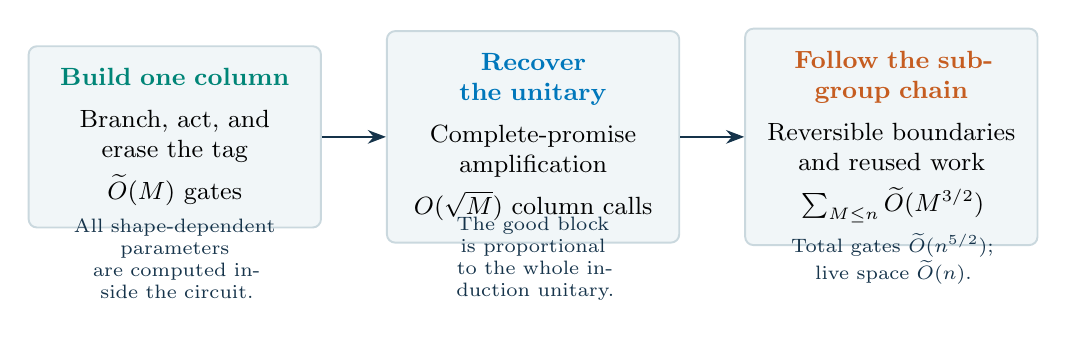
\begin{tikzpicture}[x=1cm,y=1cm]
\node[panel,text width=3.15cm,minimum height=1.65cm] (col) at (0,0)
  {\textcolor{Teal}{\textbf{Build one column}}\\[4pt]
   Branch, act, and erase the tag\\[4pt]
   $\softO(M)$ gates};
\node[panel,text width=3.15cm,minimum height=1.65cm] (amp) at (4.55,0)
  {\textcolor{Blue}{\textbf{Recover the unitary}}\\[4pt]
   Complete-promise amplification\\[4pt]
   $O(\sqrt M)$ column calls};
\node[panel,text width=3.15cm,minimum height=1.65cm] (sum) at (9.1,0)
  {\textcolor{Orange}{\textbf{Follow the subgroup chain}}\\[4pt]
   Reversible boundaries and reused work\\[4pt]
   $\sum_{M\le n}\softO(M^{3/2})$};
\draw[flow] (col.east) -- (amp.west);
\draw[flow] (amp.east) -- (sum.west);
\node[smalllabel,text width=3.4cm] at (0,-1.55)
  {All shape-dependent parameters\\are computed inside the circuit.};
\node[smalllabel,text width=3.4cm] at (4.55,-1.55)
  {The good block is proportional\\to the whole induction unitary.};
\node[smalllabel,text width=3.4cm] at (9.1,-1.55)
  {Total gates $\softO(n^{5/2})$;\\live space $\softO(n)$.};
\end{tikzpicture}
\caption{The argument in three scales. The first two boxes implement one
induction level. The final box sums levels, not separate copies of their
workspace. No measurement or postselection occurs.}\label{fig:overview}
\end{figure}

\subsection{Relation to previous constructions}\label{sec:related}

The subgroup chain
$S_1\subset S_2\subset\cdots\subset S_n$
and its multiplicity-free branching rule organize both the established
algorithms and this construction~\cite{beals,mrr,bgo,toolbox}.
In the Beals-style implementation developed by Bruinsma, Grinko, and
Ozols, successor-state preparation and controlled transversal
representations already appear~\cite[Section 4 and Appendix A.2]{bgo}.
Their implementation assembles induction by processing transversal
elements sequentially. We instead retain the transversal index, erase it
in a uniform basis, and amplify the resulting unitary block.
Sorting-network corner extraction also appears in their
Appendix A.3.1. We do not claim these individual primitives as new.

The amplification step uses the oblivious-amplification principle of
Berry et al.~\cite[Lemma 3.6]{oaa}. Our formulation isolates the two
different promise subspaces and makes clear why source-isometry
approximation suffices: the image reflection depends only on the
prepared source subspace, not on an arbitrary completion of its unitary.
Finite synthesis is also standard~\cite{sk,mw}. Theorem 4.5 of
van Melkebeek and Watson supplies the finite-precision \emph{bit-model}
uniformity needed here~\cite{mw}.

A separate line concerns the quantum character transform (QCT).
Rathore and Zhou obtain a $\softO(n^{5/2})$-gate, $O(n)$-qubit QCT
using Hamiltonian methods~\cite[Theorem 5.1]{rz}.
The QCT, also studied in~\cite{qct},
acts on conjugacy-class and irreducible-character labels.
It is a different task from the full $n!$-dimensional QFT, whose output
includes \emph{both} representation-matrix indices.
Consequently, a matching exponent for the QCT does not establish the
full-QFT bound proved here. Conversely, generic preparation, erasure,
or amplification ideas should not be attributed exclusively to this work.

\begin{table}[t]
\centering
\small
\begin{tabularx}{\textwidth}{@{}Xlll@{}}
\toprule
Construction & Transform & Gates & Live qubits\\
\midrule
Bruinsma--Grinko--Ozols~\cite[Thm.\ 1.1]{bgo}
 & Full QFT & $\softO(n^3)$ & $\softO(n^{3/2})$\\
Rathore--Zhou~\cite[Thm.\ 5.1]{rz}
 & Character transform & $\softO(n^{5/2})$ & $O(n)$\\
This work, Theorem~\ref{thm:main}
 & Full QFT & $\softO(n^{5/2})$ & $\softO(n)$\\
\bottomrule
\end{tabularx}
\caption{Scope matters as well as the exponent. The first and last rows
concern the full Fourier transform. The middle row concerns a different,
smaller transform and is included to delimit the claim, not as a
like-for-like runtime comparison. The first row reproduces a stated
theorem bound, not a space lower bound. The character-transform estimate
is for inverse-polynomial error. Prior rows count one-/two-qubit gates;
our row includes finite-gate synthesis.}\label{tab:comparison}
\end{table}

\subsection{How to read the proof}

Figure~\ref{fig:overview} gives the cost argument before its implementation
details. Section~\ref{sec:conventions} fixes the encodings and error model.
Section~\ref{sec:induction} introduces the induction map through a worked
four-box example. Sections~\ref{sec:bookkeeping}--\ref{sec:generators}
construct a near-linear column circuit.
Section~\ref{sec:oaa} explains the coherent amplification, and
Section~\ref{sec:composition} assembles the full transform.
Readers interested in bit complexity can then inspect the explicit
precision ledger in Section~\ref{sec:explicitcosts}.
The final sections separate the analytic guarantee from the prototype
and state the remaining implementation limitations.

\section{The transform, its encodings, and its error model}\label{sec:conventions}

The group $S_n$ consists of all permutations of $n$ objects, with
composition as its product. A representation assigns to each permutation
$g$ a matrix $R(g)$ so that $R(gh)=R(g)R(h)$. An irreducible representation
has no nontrivial invariant subspace. For $S_n$, these basic matrix
representations are indexed by partitions of $n$. The Fourier transform
reorganizes a function, or a quantum amplitude vector, into their matrix
coefficients.

A partition $\lambda\vdash m$ is a nonincreasing list of positive integers
with sum $m$. Its boxes have coordinates $(r,c)$, where $1\le c\le\lambda_r$,
and content $c-r$. A standard Young tableau fills the boxes by $1,\ldots,m$
in increasing order along every row and column. Write $d_\lambda=|\SYT(\lambda)|$.
We encode a tableau by its row word $P=(p_1,\ldots,p_m)$: label $j$ is in
row $p_j$. Its column is the within-row rank
\[
 c_j=|\{h\le j:p_h=p_j\}|.
\]
The endpoint shape is stored as a zero-padded list of row lengths, not in a
succinct or random-access data structure. Every word has $O(\log(n+1))$ bits.

Let $R_\lambda$ denote Young's real orthogonal representation, with positive
off-diagonal entries for adjacent transpositions. With the rightmost
permutation acting first, our Fourier convention is
\begin{equation}\label{eq:qft}
 \F_n\ket g=\sum_{\lambda\vdash n}\sum_{Q,R\in\SYT(\lambda)}
 \sqrt{\frac{d_\lambda}{n!}}\,
 \bra Q R_\lambda(g)\ket R\,\ket{\lambda,Q,R}.
\end{equation}
The shape register is redundant but is retained. Inputs use the unique
transversal word
\[
 g=t_{i_n}^{(n)}\cdots t_{i_1}^{(1)},\qquad
 t_i^{(M)}=(i,i+1,\ldots,M),\quad 1\le i_M\le M.
\]
The valid input and output subspaces have dimension $n!$. A circuit has an
arbitrary unitary extension on other physical bitstrings.

\paragraph{Linear-algebra conventions.}
A ket $\ket x$ denotes a basis vector, and a superposition is a linear
combination of such vectors. A unitary preserves all inner products.
An isometry $I$ satisfies $I^\dagger I=\Id$: it embeds a smaller logical
space into a larger physical space, for example by appending zero work
qubits. Its image projector is $II^\dagger$. A reflection
$2II^\dagger-\Id$ acts as $+1$ on that image and $-1$ on its orthogonal
complement. The operator norm $\norm A=\sup_{\norm\psi=1}\norm{A\psi}$
measures worst-case vector error. The channel diamond norm additionally
allows entanglement with an arbitrary untouched reference system.

We count gates from a fixed finite universal set, for example Clifford+$T$,
including reversible arithmetic and rotation synthesis. There is no QRAM,
precomputed shape oracle, free real-number arithmetic, or postselection.
The public parameters are $n$ and an integer requested precision. All loops,
capacities, and wire addresses are fixed by these parameters. A clean-error
bound means operator norm on the valid input subspace with all auxiliary
registers zero, comparing against the ideal output with auxiliaries zero.
It therefore includes leakage into auxiliary registers and holds with an
arbitrary entangled reference system. Approximate cleanup means this norm
bound, not an assertion that every synthesized circuit ends with exactly
zero auxiliary bits.

\begin{theorem}[Main bound]\label{thm:main}
For $n\ge1$ and $0<\epsilon\le1/2$ there is a uniform finite-gate circuit
with clean-input isometry $\widetilde V_n$ such that
\[
 \norm{\widetilde V_n-(\F_n\otimes\ket0_{\rm work})}\le\epsilon/2.
\]
Its elementary-gate count and maximum number of live qubits are respectively
\[
 n^{5/2}\poly(\log(n+1),\log(1/\epsilon)),\qquad
 n\poly(\log(n+1),\log(1/\epsilon)).
\]
After discarding work, the channel is within diamond distance $\epsilon$
of the ideal channel on the input promise. The same dominant bound holds
for a one-line permutation input after a reversible polynomial-logarithmic
overhead, quadratic-time encoding conversion.
\end{theorem}

The $\widetilde O$ notation below suppresses polynomial factors in
$\log(n+1)$ and $\log(1/\epsilon)$; it is not uniform in unbounded exact-real
precision. The result is an approximation theorem, not an exact finite-gate
realization. The proof optimizes the power of $n$, not the logarithmic
exponents or practical constants.

\paragraph{What coherence requires.}
For a classical shape, one could calculate an angle and then choose a
rotation. Here the input may contain $\sum_\lambda a_\lambda\ket\lambda$.
Measuring $\lambda$ would destroy its relative phases. The implementation
must instead compute
$\ket\lambda\ket0\mapsto\ket\lambda\ket{\widetilde\theta_\lambda}$,
apply the bit-controlled rotation, and erase the angle register.
The theorem counts all three operations. The classical compiler sees only
$n$ and the requested error, never the quantum shape.

\paragraph{The channel's domain.}
Let $\mathcal H_{\rm in}$ be the abstract space with orthonormal basis
$\{\ket g:g\in S_n\}$, embedded into the valid transversal encodings.
Both channels in the theorem have domain $\mathcal L(\mathcal H_{\rm in})$.
The diamond-norm comparison includes arbitrary reference systems on this
domain. No approximation to a prescribed map is claimed on invalid
physical bitstrings.

\section{The induction transform: one box at a time}\label{sec:induction}

Fix $\lambda\vdash M-1$. The notation $\mu\succ\lambda$ means that $\mu$
is obtained by adding one box to $\lambda$. If $P\in\SYT(\lambda)$, write
$P\to\mu$ for the tableau obtained by placing $M$ in that box. Define
\begin{equation}\label{eq:induction}
 (F_\lambda)_{(\mu,Q),(i,P)}=
 \sqrt{\frac{d_\mu}{M d_\lambda}}\,
 \bra Q R_\mu(t_i^{(M)})\ket{P\to\mu}.
\end{equation}
The standard multiplicity-free induction rule says that this is a unitary
map from $\mathbb C^M\otimes\mathbb C^{d_\lambda}$ to
$\bigoplus_{\mu\succ\lambda}\mathbb C^{d_\mu}$. In particular,
$\sum_{\mu\succ\lambda}d_\mu=M d_\lambda$. These representation-theoretic
facts, and the resulting QFT recurrence, are established ingredients, not
claims of this paper; see Definition 3.6, Lemma 3.7, and Theorem 3.8 of
\cite{bgo}. We prove the recurrence's circuit and error costs below.

For clarity, the induction identity can be understood by decomposing
$\operatorname{Ind}_{S_{M-1}}^{S_M}R_\lambda$. In the coset basis it has
labels $(i,P)$. Each successor representation occurs once, its restricted
$\lambda$ sector has basis $P\to\mu$, and the matrix coefficients of the
intertwiner are \eqref{eq:induction}. Orthogonality fixes the normalization.
This is the only non-elementary representation-theoretic input to the
induction map itself.

\subsection{A four-box example}\label{sec:example}

Take $M=4$ and $\lambda=(2,1)$. There are two standard tableaux of shape
$\lambda$. Its three successors are $(3,1)$, $(2,2)$, and $(2,1,1)$,
with dimensions $3,2,3$. The branching probabilities are consequently
$3/8,1/4,3/8$. For a particular tableau $P$, the preparation $B$ appends
the label $4$ in the three possible boxes, with the square roots of these
probabilities as amplitudes (Figure~\ref{fig:young}).
The displayed tableau has row word $(1,1,2)$ and column cache $(1,2,1)$.
Its successors append row labels $1$, $2$, and $3$, respectively.
This eight-dimensional fixed-$\lambda$ induction block is one part of the
construction, not the full $24$-dimensional Fourier transform over $S_4$.

\begin{figure}[htbp]
\centering
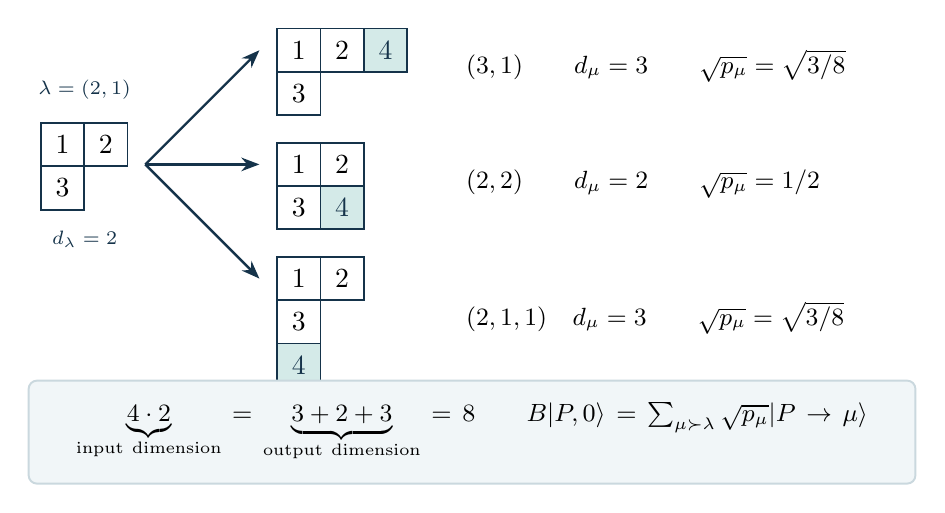
\begin{tikzpicture}[x=1cm,y=1cm]
\begin{scope}[shift={(0,0)}]
\node[cell] at (0,0) {$1$};
\node[cell] at (.55,0) {$2$};
\node[cell] at (0,-.55) {$3$};
\node[smalllabel] at (.28,.7) {$\lambda=(2,1)$};
\node[smalllabel] at (.28,-1.2) {$d_\lambda=2$};
\end{scope}
\draw[flow] (1.05,-.25) -- (2.5,1.2);
\draw[flow] (1.05,-.25) -- (2.5,-.25);
\draw[flow] (1.05,-.25) -- (2.5,-1.7);
\begin{scope}[shift={(3,1.2)}]
\node[cell] at (0,0) {$1$};
\node[cell] at (.55,0) {$2$};
\node[added] at (1.1,0) {$4$};
\node[cell] at (0,-.55) {$3$};
\end{scope}
\begin{scope}[shift={(3,-.25)}]
\node[cell] at (0,0) {$1$};
\node[cell] at (.55,0) {$2$};
\node[cell] at (0,-.55) {$3$};
\node[added] at (.55,-.55) {$4$};
\end{scope}
\begin{scope}[shift={(3,-1.7)}]
\node[cell] at (0,0) {$1$};
\node[cell] at (.55,0) {$2$};
\node[cell] at (0,-.55) {$3$};
\node[added] at (0,-1.1) {$4$};
\end{scope}
\node[anchor=west,font=\small] at (5,1.0)
  {$(3,1)\qquad d_\mu=3\qquad \sqrt{p_\mu}=\sqrt{3/8}$};
\node[anchor=west,font=\small] at (5,-.5)
  {$(2,2)\qquad d_\mu=2\qquad \sqrt{p_\mu}=1/2$};
\node[anchor=west,font=\small] at (5,-2.2)
  {$(2,1,1)\quad d_\mu=3\qquad \sqrt{p_\mu}=\sqrt{3/8}$};
\node[panel,text width=10.7cm] at (5.2,-3.65)
  {$\underbrace{4\cdot2}_{\text{input dimension}}
   =\underbrace{3+2+3}_{\text{output dimension}}=8
   \qquad
   B\ket{P,0}=\sum_{\mu\succ\lambda}\sqrt{p_\mu}\ket{P\to\mu}$};
\end{tikzpicture}
\caption{Branching at the first three-successor shape. A highlighted box
contains the new label, not a measured choice. The preparation is coherent
over the three successors and over the two possible input tableaux.
The probabilities are dimension ratios, not a uniform distribution over
successor shapes.}\label{fig:young}
\end{figure}

This preparation is only the first part of induction. The tag
$i\in\{1,2,3,4\}$ selects the permutation $t_i$, whose representation
acts on the enlarged tableau. Erasing the tag in a uniform basis then
produces the matrix block $F_\lambda/2$. A single successful block would
have probability $1/4$ on any normalized input. The algorithm does not
measure that block. It amplifies it coherently, preserving superpositions
of tags, tableaux, and shapes.

The distinction between a prepared column and a unitary is worth keeping
in view. Preparing the right output for one classical input does not by
itself implement the linear transformation on an unknown superposition.
Retaining the tag makes different tag sectors orthogonal; within each
sector the column map is an isometry. The clean map therefore extends to
a unitary. Coherent tag erasure and the exact unitary block identity are
what make amplification possible.

\subsection{A common physical register space}

At a fixed stage $M$, the unchanged external register stores $\lambda$ in
$M$ padded row-length slots. There are a tag register with alphabet
$\{0,\ldots,M\}$, $M$ tableau row slots, an attenuation flag, and work
registers. The tag value $0$ and row value $0$ are reserved as blanks.
Define isometries $I_\lambda,J_\lambda$ into this same physical space:
\begin{align*}
 I_\lambda\ket{i,P}&=\ket{\lambda;i,P,0;0;0_{W}},\quad 1\le i\le M,\\
 J_\lambda\ket{\mu,Q}&=\ket{\lambda;0,Q;0;0_{W}},\quad\mu\succ\lambda.
\end{align*}
Here $0_W$ includes \emph{all} work used by the column unitary, including
coefficient, angle, column-cache, and sorting registers. The external shape
is part of the control, not an erased output. Define $I,J,F$ by direct sum
over valid $\lambda$. Their ranks vary by shape, but their physical wire
counts do not. Right tableaux and unused future input tags are spectators;
they are not tested for zero. Inactive tails of larger-capacity stage
registers are also untouched spectators, initially zero.

Two reflections will be required on these \emph{full} promises:
\begin{equation}\label{eq:reflect}
 R_I=2II^\dagger-\Id,\qquad R_J=2JJ^\dagger-\Id.
\end{equation}
Testing only the tag is not sufficient. Dedicated predicate helper registers
are kept separate from $W$-work and return exactly to zero after each
reflection. All identities involving these reflections are on the invariant
subspace where those dedicated helpers start at zero.

\begin{table}[htbp]
\centering\small
\begin{tabularx}{\textwidth}{@{}lXX@{}}
\toprule
Register & Role during a column call & Promise-reflection treatment\\
\midrule
Shape $\lambda$ & Coherent control; unchanged & Valid size-$(M-1)$ partition\\
Tag and left tableau & Input $(i,P)$; output $(0,Q)$ & Full source or target validity\\
Attenuation flag & Sets the known block amplitude & Must be zero\\
Column work $W$ & Arithmetic, cache, sorting history & Every active work bit must be zero\\
Predicate helpers & Used only by the reflections & Start clean; uncomputed exactly\\
Right tableau, future tags & Untouched spectators & Not tested for zero\\
\bottomrule
\end{tabularx}
\caption{Which registers belong to the promise? The distinction prevents
two errors: reflecting only on a zero tag, and accidentally rejecting
nonzero spectator data.}\label{tab:registers}
\end{table}

\section{Near-linear reversible tableau bookkeeping}\label{sec:bookkeeping}

\begin{lemma}[Fixed-schedule word operations]\label{lem:words}
For row words and padded shapes with $M$ slots, the following functions have
clean reversible XOR implementations using $M\poly(\log(n+1))$ gates and
work bits: within-row column ranks, endpoint row histograms, standard-tableau
validity, partition validity, and the condition $\mu\succ\lambda$.
Consequently the reflections \eqref{eq:reflect}, including zero tests of
$W$-work of size $M\poly(\log(n+1),\log(1/\eta))$, have cost and helper
space $M\poly(\log(n+1),\log(1/\eta))$.
\end{lemma}

\begin{proof}
Use a fixed bitonic sorting network on a power-of-two padding of $O(M)$
records. Its $O(M\log^2(M+1))$ compare-exchanges compare $O(\log(n+1))$-bit
keys and retain their comparison bits. Sentinels and original-position
labels are included in the keys, so every comparison is deterministic,
including on equal or malformed data. Reversing swaps and comparisons
restores the records and zeros the comparison bits. A scan uses a fresh
output word at each step and retains its old words until reversal. Modular
fixed-width arithmetic gives a total Boolean function on every input;
valid inputs fit in the chosen capacities.
For predicates, accumulator widths are chosen for \emph{all physical
encodings}, not only valid tableaux. A sum of $M$ unsigned $w$-bit
row lengths uses $w+\lceil\log_2 M\rceil+1$ bits, and differences are
signed and widened. Alternatively, an overflow flag is retained and
rejected. Thus wraparound cannot turn a malformed shape into an accepted
partition or cover. All these widths remain $O(\log(n+1))$.

For columns, sort records $(p_j,j)$ by row and then label. A segmented
prefix count gives the rank of each label within its row. Sorting by
original label places the resulting ranks at public output addresses.
For the histogram, insert one sentinel for each row $r=1,\ldots,M$ after
that row's data records. Its segmented count is the row length; sort these
sentinels by their public row labels for extraction. Check separately that
all input rows lie in $[1,M]$. The row histogram must be nonincreasing.
To test tableau validity, sort label records by their computed column and
then row. Within each column, check that rows are consecutive starting at
one and that labels increase. Within-row labels already increase by the
definition of a row word. This proves necessity and sufficiency, including
absence of holes. Partition validity is a fixed scan of row comparisons,
nonnegativity, and the total sum. Cover validity checks that the padded
rowwise differences are zero except for one $+1$, with both partitions
valid and the correct total sizes.

Each algorithm is made into a clean function oracle by computing its
intermediate history, copying the requested outputs by XOR, and reversing
the history. Thus it works even when the target XOR register is nonzero.
Malformed input is not an excuse to drop information: its computed
predicate is copied, then the same computation is reversed. No lookup by a
data-dependent row address is used.

For $R_I$, test all of the following: $\lambda$ is a partition of $M-1$;
the first $M-1$ row symbols encode a standard tableau whose endpoint is
exactly $\lambda$; the final row symbol is zero; $1\le i\le M$; and the
attenuation flag and every $W$-work bit are zero. For $R_J$, test that
$\lambda\vdash M-1$, all $M$ row symbols encode a standard tableau $Q$
whose endpoint $\mu$ covers $\lambda$, and the tag, flag, and every
$W$-work bit are zero. Untested right paths and future digits are
tensor-identity spectator factors in both projectors.
Compute the conjunction in
separate clean helper space, apply phase $-1$ precisely when it is false,
and uncompute. All this is exact reversible Boolean logic. The helpers
are \emph{not} borrowed from possibly dirty $W$-work.
\end{proof}

One bookkeeping point is essential later: the column cache is built by a
\emph{clean} XOR oracle before applying representation matrices. We do not
leave sorting history attached to the old tableau. After the tableau
changes, the same XOR oracle evaluated on the new tableau erases the
updated cache.

\section{Elementary coherent branching coefficients}\label{sec:weights}

Let $x_0>y_0>x_1>\cdots>y_{k-2}>x_{k-1}$ be the integer contents of
addable and removable boxes of $\lambda$, respectively. The standard
dimension-ratio identity gives, for the successor belonging to $x_i$,
\begin{equation}\label{eq:residue}
 p_i=\frac{d_{\lambda+\Box_i}}{M d_\lambda}
 =\frac{\prod_{j=0}^{k-2}|x_i-y_j|}{\prod_{h\ne i}|x_i-x_h|}.
\end{equation}
See also Lemma 2.4 of \cite{bgo}. Normalization follows directly by taking
the coefficient of $1/z$ in the partial fractions of
$\prod_j(z-y_j)/\prod_i(z-x_i)$. A scan of padded row lengths identifies
corners; a fixed stable compaction by sorting puts active corners first.
There are $k$ addable corners and $k-1$ removable corners, with
\[
 \frac{k(k-1)}2\le M-1,\qquad L:=x_0-x_{k-1}\le2M.
\]
Indeed $k-1$ distinct positive row lengths require at least
$1+\cdots+(k-1)$ boxes. Thus all arrays may be padded to the public
least power-of-two capacity
$K=2^{\lceil\log_2(\lceil\sqrt{2M}\rceil+1)\rceil}$, so $K^2=O(M)$.

\begin{lemma}[Bounded products and precision]\label{lem:precision}
For $k>1$, each probability in \eqref{eq:residue} has the factorization
\begin{equation}\label{eq:bounded}
 p_i=\prod_{j<i}\frac{y_j-x_i}{x_j-x_i}
       \prod_{j\ge i}\frac{x_i-y_j}{x_i-x_{j+1}},
\end{equation}
with every factor strictly between zero and one, and $p_i\ge L^{-2}$.
For each $i$ start with $N_i^{(0)}=2^b$ and, for a factor $a/d$, update
\[
 N_i^{(t+1)}=\left\lfloor N_i^{(t)}a/d\right\rfloor.
\]
Writing $N_i=N_i^{(k-1)}$, $T=\sum_iN_i$, and $\widehat p_i=N_i/T$,
the following bounds hold whenever the stated precision makes $T>0$:
\begin{align}
 0\le p_i-2^{-b}N_i&<(k-1)2^{-b},\label{eq:round}\\
 \norm{p-\widehat p}_1&\le2k(k-1)2^{-b},\label{eq:l1}\\
 \left\|\sum_i(\sqrt{p_i}-\sqrt{\widehat p_i})\ket i\right\|
 &\le\sqrt{2k(k-1)2^{-b}}.\label{eq:root}
\end{align}
In particular $b=O(\log(M+1)+\log(1/\eta))$ suffices for a clean
coherent preparation of $\sum_i\sqrt{p_i}\ket i$ with error at most $\eta$
and $M\poly(\log(n+1),\log(1/\eta))$ elementary gates and work bits.
The case $k=1$ is an exact deterministic state.
\end{lemma}

\begin{proof}
Regrouping denominators gives \eqref{eq:bounded}. On the left of $i$, use
$y_j\ge x_{j+1}+1$, and telescope all but the last positive integer
numerator, giving a lower bound $1/(x_0-x_i)$ when this side is nonempty.
On the right, use $y_j\le x_j-1$ and obtain $1/(x_i-x_{k-1})$ in the
same way. An empty side contributes one. This proves $p_i\ge L^{-2}$.
Each rounded update contracts the previous error and adds less than $2^{-b}$,
proving \eqref{eq:round}. If
$\Delta=1-2^{-b}\sum_iN_i$, then
$0\le\Delta\le k(k-1)2^{-b}$. Renormalization changes the dyadic vector
by exactly $\Delta$ in $\ell^1$, proving \eqref{eq:l1}.
The inequality $(\sqrt a-\sqrt b)^2\le|a-b|$ proves \eqref{eq:root}.

For example, take the public precision
\[
 b\ge\max\left\{\left\lceil\log_2(2(K-1)(2M)^2)\right\rceil,
             2\left\lceil\log_2(4K/\eta)\right\rceil\right\}.
\]
The weight loss is at most $(K-1)2^{-b}\le1/[2(2M)^2]\le p_i/2$,
so every active $N_i$ is positive. Weight-rounding state error is less
than $\eta/2$. Inactive leaves are exactly zero. Throughout an update
$N_i\le2^b$ and its product with a numerator is at most $2^bL$; there
are no exponentially large intermediate products. Fixed multiplication
and division use polynomially many gates in $b+\log(M+1)$. Compute one
product history, copy its final word, and reverse that history before
moving to the next $i$. This uses $O(K^2)$ updates and $O(K)$ words of
history at a time, up to polynomial word-arithmetic overhead.

Build the binary tree of the integer masses $N_i$. This uses the familiar
conditional-mass preparation pattern~\cite{gr}, with the present integer
weights and explicit rounding bounds. Each mass is at most
$K2^b$. At a node with child masses $A,B$, use the real rotation of angle
$\theta=\operatorname{atan2}(\sqrt B,\sqrt A)$, controlled by the already
prepared prefix. Zero children use exact identity or bit-flip endpoints;
a zero parent uses identity. There are $K-1$ fixed nodes. Compute each
angle to error at most $\eta/(8K)$ and synthesize its controlled rotation
to operator error at most $\eta/(8K)$. Telescoping the gates gives error
at most $\eta/4$, leaving slack in the claimed bound. Each node's prefix
condition uses at most $\log_2 K$ bits: compute its equality flag in clean
helper bits, apply the controlled rotation, and uncompute the flag. This
adds only polynomial-logarithmic cost per node, with reusable helper space.

These angle computations need no oracle: evaluate
$z=\sqrt{\min(A,B)/\max(A,B)}\in[0,1]$ by integer division and a fixed
integer-square-root routine to enough dyadic places. For $z\le1/2$ the
alternating series for $\atan z$ converges geometrically. For $z>1/2$ use
$\atan z=\pi/4-\atan((1-z)/(1+z))$; the new argument is at most $1/3$.
Machin's formula computes $\pi/4=4\atan(1/5)-\atan(1/239)$ to the same
accuracy. Put $c=O(\log(K/\eta))$. Evaluate the $O(c)$ terms by fixed-point
Horner evaluation, rounding each operation at $c+O(\log c)$ fractional
bits; these guard bits bound the accumulated arithmetic error by $O(2^{-c})$.
Exact rational powers are useful reference certificates but are not the
claimed bounded-word circuit implementation.
The square-root input can be evaluated to twice the desired output bits,
using $|\sqrt u-\sqrt v|\le\sqrt{|u-v|}$. If $B>A$, subtract the small
angle from $\pi/2$. Every step has polynomial bit complexity.

The $O(c)$ angle bits control $O(c)$ fixed dyadic rotations. Assign each
bit-controlled rotation synthesis error $O(\eta/(Kc))$; their sum is
$O(\eta/K)$ per tree node. Finite-gate synthesis has
polynomial-logarithmic word length \cite{sk}. For classical compilation
in a finite-precision bit model we use Theorem 4.5 of \cite{mw}, rather
than interpreting an arithmetic-operation count as a bit-complexity bound.
The approximation here is of the actual controlled gate in matrix norm,
not merely a one-qubit operation up to an uncontrolled global phase.
For instance a controlled real rotation decomposes into two CNOTs and a
half-angle rotation paired with its exact circuit adjoint; its irrelevant
single-qubit synthesis phase then cancels. Prefix and angle-bit conjunctions
are computed and uncomputed by exact Boolean circuits. Their cost is
included in the polynomial-logarithmic factor.
Compute, rotate, and uncompute the angle
scratch. Tree masses, weight words, and contents are erased from the
unchanged shape after preparation. The loop bounds use $K$, not the
data-dependent $k$. Dummy factors are one, dummy leaves zero, and all
invalid denominators are replaced by one in totalized arithmetic. A
shape-validity guard may select a fixed default state on invalid shapes.
All controlled maps therefore have a unitary extension, with no need to
specialize or enumerate circuits over partitions.
\end{proof}

To obtain the actual added row rather than its corner ordinal, use a fixed
scan of the $K$ corner records: controlled on ordinal equality, XOR the
selected row into the final blank tableau slot. A second fixed scan,
controlled on equality with that unique row, erases the ordinal. This is
reversible on the prepared support. On the complement it is still a
composition of reversible XOR gates. The parameter table is then erased
using the unchanged $\lambda$. Thus Lemma~\ref{lem:precision} implements
the branching column map
\begin{equation}\label{eq:B}
 B:\ket{P,0}\longmapsto
 \sum_{\mu\succ\lambda}\sqrt{d_\mu/(M d_\lambda)}\ket{P\to\mu}
\end{equation}
with the same clean-error and cost bounds. A fixed-angle approximate
circuit can leak into padded states; its entire leakage is included in the
isometry error, not assumed to vanish exactly.

\section{The selected transversal in near-linear cost}\label{sec:generators}

Write $s_j=(j,j+1)$ and $d=\cont(j+1)-\cont(j)$ in a valid tableau.
Young's orthogonal rule is
\[
 R_\mu(s_j)\ket P=d^{-1}\ket P+
 \sqrt{1-d^{-2}}\ket{s_jP}.
\]
When $|d|=1$ the second term is absent and the action is the exact sign $d$.
Otherwise $s_jP$ is standard and its axial distance is $-d$.

\begin{lemma}[Cached generators]\label{lem:generators}
With a correct column cache, one public-index Young generator, also
controlled on a public comparison with the tag, can be implemented to
operator error $\zeta$ on the valid-tableau/cache subspace in
$\poly(\log(n+1),\log(1/\zeta))$ gates and work bits. The ideal operation
preserves that subspace and updates the column cache correctly.
\end{lemma}

\begin{proof}
Only the two records $(p_j,c_j)$ and $(p_{j+1},c_{j+1})$ are accessed.
For $|d|>1$, compute $f=[d<0]$ and swap both records if $f=1$, thereby
canonicalizing the pair to a positive distance $D=|d|$. Retain $f$; this
step must not discard which member of the pair was present. On $f$ apply
\[
 A_D=\begin{pmatrix}1/D&\sqrt{1-D^{-2}}\\
             \sqrt{1-D^{-2}}&-1/D\end{pmatrix}
       =R_y(2\arccos(1/D))Z.
\]
Compute and erase $D$ and the angle while the canonical records are
unchanged. Undo the record swap controlled on the now-superposed $f$.
Finally XOR $[d_{\rm final}<0]$ into $f$, erasing it on both branches.
The $|d|=1$ branch applies the exact sign; its guard is invariant and can
be erased. On invalid inputs use safe total arithmetic and a reversible
extension of this gate sequence, without making a promise of cleanup.

The swapped column cache is correct because $s_jP$ interchanges the boxes
containing $j,j+1$; all other box coordinates are unchanged. If
$\theta=\arccos(1/D)$, then
$\norm{A_D(\theta)-A_D(\widetilde\theta)}
=2|\sin((\theta-\widetilde\theta)/2)|\le|\theta-\widetilde\theta|$.
Compute $\theta$ by the same bounded-ratio square-root/arctangent routine
as above, or via $\pi/2-\atan(1/\sqrt{D^2-1})$. The latter ratio is at
most $1/\sqrt3$; a further range reduction gives a geometrically
convergent series. Word precision $O(\log(n+1)+\log(1/\zeta))$ suffices.
Arithmetic is uncomputed and controlled dyadic rotations are synthesized
with the claimed polynomial-logarithmic cost. For a $c$-bit angle word,
assign each of its $O(c)$ controlled constant rotations error $O(\zeta/c)$,
using the same phase-aware construction as above. The axial-distance
sectors are orthogonal controls, so the error is the maximum sector error,
not a sum over tableaux. Only the subsequent $M-1$ generator applications
are summed; $\zeta=O(\eta/M)$ suffices for the selected transversal.
\end{proof}

Build the clean column cache of the complete $M$-box tableau, then, in
chronological order $j=M-1,M-2,\ldots,1$, apply this generator controlled
on $[i\le j]$. Since $t_i=s_i s_{i+1}\cdots s_{M-1}$, this order implements
\[
 V:\ket{i,Q}\longmapsto\ket i R_\mu(t_i)\ket Q.
\]
The tag zero case can act as identity. The cache is updated at each swap,
and is erased by the clean column XOR oracle evaluated on the final
tableau, not by reversing stale pre-generator history. With per-generator
error $O(\eta/M)$, the whole selected operation has clean error $O(\eta)$
and cost $M\poly(\log(n+1),\log(1/\eta))$. This error statement follows
by telescoping on ideal intermediate valid-cache subspaces; it does not
require approximate intermediate states to satisfy exact validity.

\section{Column erasure and full-unitary amplification}\label{sec:oaa}

Let $H_M$ be the specific tag unitary defined by a fixed binary preparation
tree, with $H_M\ket0=M^{-1/2}\sum_{i=1}^M\ket i$. The tree has $O(M)$
leaves; approximating each of its fixed rotations gives a whole-unitary
operator-norm approximation of $H_M$, and hence of its adjoint, to error
$\eta$ in $M\poly(\log(n+1),\log(1/\eta))$ gates.
No stronger cost bound for this elementary uniform
state is needed. Define the ideal unitary
\[
 W_0=(H_M^\dagger\otimes\Id)VB.
\]
Projecting onto tag zero and all work zero gives the exact block identity
\begin{equation}\label{eq:block}
 J^\dagger W_0 I=F/\sqrt M.
\end{equation}
Projection here specifies a matrix block; it is not a measurement.

The bra of the uniform tag state contributes the same factor
$1/\sqrt M$ to every retained tag. The remaining coefficients are exactly
those in \eqref{eq:induction}. Thus the good block is a scalar multiple
of a unitary on \emph{every} input, not merely a state with a large overlap
for one chosen column. This input-independent normalization is what
oblivious amplification needs.

Choose public values
\begin{equation}\label{eq:attenuate}
 r_M=\lceil\sqrt M\rceil,\qquad
 \theta_M=\frac{\pi}{4r_M+2},\qquad a_M=\sqrt M\sin\theta_M.
\end{equation}
Since $a_M\le\pi/4<1$, a one-qubit flag rotation with zero amplitude $a_M$
is legal. Apply it in addition to $W_0$ and call the result $W$.
The target tests flag zero, giving
\begin{equation}\label{eq:attenuated}
 J^\dagger W I=\sin\theta_M F.
\end{equation}
Computing and synthesizing this public angle has polynomial-logarithmic
cost. Special-case $M=1$ as a trivial induction if desired.

\begin{lemma}[Two-promise OAA and its error]\label{lem:oaa}
Suppose $I,J$ are isometries, $F$ is unitary between their equal-dimensional
domains, and a unitary $W$ obeys $J^\dagger WI=\sin\theta F$ with
$\theta=\pi/(4r+2)$ for an integer $r\ge1$. Then
\begin{equation}\label{eq:exactoaa}
 (-WR_IW^\dagger R_J)^r WI=JF.
\end{equation}
If $\widetilde W$ is unitary and
$\norm{(\widetilde W-W)I}\le\eta$, keeping the exact promise reflections
gives clean output error at most $(4r+1)\eta$.
\end{lemma}

\begin{proof}
Put $A=WI$, $G=JF$, $s=\sin\theta$, $c=\cos\theta$, and
$C=(A-sG)/c$. The block identity implies $G^\dagger C=0$ and
$C^\dagger C=\Id$, with $A=sG+cC$. In particular $J^\dagger C=0$.
On each corresponding two-dimensional plane,
$-WR_IW^\dagger R_J=-(2AA^\dagger-\Id)(2JJ^\dagger-\Id)$ sends
\[
 G\mapsto\cos(2\theta)G-\sin(2\theta)C,\qquad
 C\mapsto\sin(2\theta)G+\cos(2\theta)C.
\]
Its $r$th power applied to $A$ is
$\sin((2r+1)\theta)G+\cos((2r+1)\theta)C=G$.
The minus sign in \eqref{eq:exactoaa} is included; it avoids an unwanted
phase convention. This is the usual oblivious-amplification geometry
\cite{oaa}, written for distinct complete source and target promises.

For the error bound, set $\widetilde A=\widetilde W I$. Then
$\norm{\widetilde A\widetilde A^\dagger-AA^\dagger}\le2\eta$,
so the two image reflections differ by at most $4\eta$. Telescoping
the $r$ rounds and the initial isometry gives $(4r+1)\eta$.
Only the action of $W$ on the whole source promise must be approximated;
no bound on its arbitrary unitary completion is needed. The implemented
inverse is the exact adjoint circuit $\widetilde W^\dagger$, not a
separately synthesized inverse. If the two reflections themselves had
global errors $\rho_I,\rho_J$, one would add $r(\rho_I+\rho_J)$.
Here the Boolean promise reflections are exact.
\end{proof}

\begin{figure}[htbp]
\centering
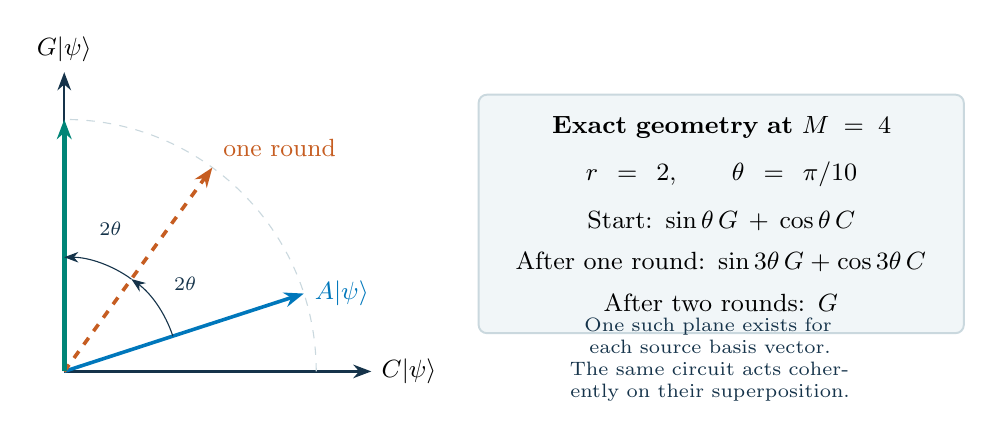
\begin{tikzpicture}[x=1cm,y=1cm]
\draw[flow] (0,0) -- (3.9,0) node[right,font=\small] {$C\ket\psi$};
\draw[flow] (0,0) -- (0,3.8) node[above,font=\small] {$G\ket\psi$};
\draw[draw=Rule,dashed] (3.2,0) arc[start angle=0,end angle=90,radius=3.2];
\draw[-{Stealth[length=2.5mm]},Blue,line width=1.3pt]
 (0,0) -- (18:3.2) node[right,font=\small] {$A\ket\psi$};
\draw[-{Stealth[length=2.5mm]},Orange,dashed,line width=1.3pt]
 (0,0) -- (54:3.2) node[above right,font=\small] {one round};
\draw[-{Stealth[length=2.5mm]},Teal,line width=1.8pt]
 (0,0) -- (90:3.2);
\draw[-{Stealth[length=1.8mm]},draw=Ink]
 (18:1.45) arc[start angle=18,end angle=54,radius=1.45];
\draw[-{Stealth[length=1.8mm]},draw=Ink]
 (54:1.45) arc[start angle=54,end angle=90,radius=1.45];
\node[smalllabel] at (36:1.9) {$2\theta$};
\node[smalllabel] at (72:1.9) {$2\theta$};
\node[panel,anchor=west,text width=5.6cm] at (5.25,2.0)
 {\textbf{Exact geometry at $M=4$}\\[6pt]
  $r=2,\qquad \theta=\pi/10$\\[6pt]
  Start: $\sin\theta\,G+\cos\theta\,C$\\[4pt]
  After one round: $\sin3\theta\,G+\cos3\theta\,C$\\[4pt]
  After two rounds: $G$};
\node[smalllabel,text width=5.6cm,anchor=west] at (5.25,.15)
 {One such plane exists for each source basis vector.\\
  The same circuit acts coherently on their superposition.};
\end{tikzpicture}
\caption{Amplification is rotation, not repeated measurement. In the
ideal construction, $G$ is the desired clean output and $C$ is an
orthogonal complement. Attenuation chooses the starting angle so an
integer number of rounds reaches $G$ exactly. Dashed and solid arrows
distinguish intermediate and initial/final states.}\label{fig:oaa}
\end{figure}

\paragraph{One induction level, in circuit order.}
The construction can be read as the following fixed schedule.
\begin{enumerate}[label=\arabic*.,leftmargin=1.6em]
\item Prepare the successor tableau with $B$, retaining the input tag.
\item Build its column cache, apply the $M-1$ selected adjacent generators,
      and erase the updated cache. This is $V$.
\item Apply $H_M^\dagger$ to the tag and the public attenuation rotation
      to the flag. Together, these operations are $W$.
\item Repeat $r_M$ times: $R_J$, $W^\dagger$, $R_I$, $W$, and the
      overall factor $-\Id$, in that chronological order.
\item Update the outer shape and right tableau as described next.
\end{enumerate}
Every inverse in step 4 is the literal adjoint of the chosen finite
circuit. None of these steps selects a measured outcome.

Lemmas~\ref{lem:words}--\ref{lem:generators}, the tag preparation, and the
flag rotation together construct $\widetilde W$ with source-isometry
error $\eta$ at cost $M\poly(\log(n+1),\log(1/\eta))$. Split this budget
among branching preparation, the selected generators, tag preparation,
and the flag. At fixed $\lambda$ the source tableau is a spectator during
branching preparation, so its state-error bound is an operator-isometry
bound. Direct sum over $\lambda$ takes a maximum of these errors, not a
sum over the number of partitions. The public capacities and number of
amplification rounds are the same for every coherent $\lambda$ sector.

There are $2r_M+1$ calls to $\widetilde W$ or its adjoint and $2r_M$
promise reflections. Thus a complete clean induction step costs
\begin{equation}\label{eq:stagecost}
 M^{3/2}\poly(\log(n+1),\log(1/\eta))
\end{equation}
gates and $M\poly(\log(n+1),\log(1/\eta))$ work bits. No branch is
postselected and no shape-dependent angle table is supplied for free.

\section{Assembling the full transform}\label{sec:composition}

At stage $M$ the previous Fourier registers have shape $\lambda$ and
tableaux $P,R\in\SYT(\lambda)$. Apply the amplified $F_\lambda$ to
$(i_M,P)$, leaving $R$ unchanged. On the ideal output, compute the new
shape $\mu$ from $Q$, and compute the unique row $a$ where $\mu-\lambda$
equals one. Append $a$ to $R$ to form $R\to\mu$.

This boundary map is clean and reversible in $\widetilde O(M)$ cost.
For example, keep the newly computed $\mu$, transfer $a$ to the blank
last right-path slot, and erase temporary difference work while $\lambda$
is still available. Then XOR the reconstructible old shape
$\mu-\Box_a$ into the old $\lambda$ register. It becomes zero. Swap the
new and old shape registers, retaining only $\mu$. The former new-shape
register is now zero. All row scans, histograms, and compute-copy-reverse
operations have fixed schedules. On malformed inputs these same XOR
operations still define a reversible circuit; residuals need not vanish.
On approximate inputs their norm is charged to the preceding error.

To verify \eqref{eq:qft} inductively, write $g=t_i^{(M)}h$ with
$h\in S_{M-1}$. The old coefficient times the induction coefficient is
\[
 \sqrt{\frac{d_\lambda}{(M-1)!}}\,
 \bra P R_\lambda(h)\ket R\,
 \sqrt{\frac{d_\mu}{M d_\lambda}}\,
 \bra Q R_\mu(t_i)\ket{P\to\mu}.
\]
Sum over $P$ and use the adapted restriction of $R_\mu$ to the
$\lambda$ sector. This is
$\sqrt{d_\mu/M!}\bra Q R_\mu(t_i h)\ket{R\to\mu}$,
exactly the next Fourier coefficient. Starting from the empty tableau
proves the whole recurrence, including the right-path update.

\begin{proof}[Proof of Theorem~\ref{thm:main}]
Use the public per-column error budget
\begin{equation}\label{eq:budget}
 \eta=\frac{\epsilon}{2n(4\lceil\sqrt n\rceil+1)}.
\end{equation}
By Lemma~\ref{lem:oaa}, the sum of clean induction errors is at most
$n(4\lceil\sqrt n\rceil+1)\eta=\epsilon/2$. Exact boundary maps do not
increase it. This hybrid argument evaluates each individual error on the
ideal valid input to that stage; actual accumulated leakage is carried
unitarily and requires no intermediate projection or measurement.
More explicitly, let $U_j$ be ideal stages including their exact
boundaries, let $\widetilde U_j$ be their implementations on the same
physical registers, and let $E_{\rm in}$ embed a valid clean input. Then
\begin{equation}\label{eq:hybrid}
\norm{(\widetilde U_m\cdots\widetilde U_1-U_m\cdots U_1)E_{\rm in}}
\le
\sum_{j=1}^m
\norm{(\widetilde U_j-U_j)U_{j-1}\cdots U_1E_{\rm in}}.
\end{equation}
The omitted approximate suffixes are unitary and cannot enlarge norms.
Each ideal prefix has clean work, so each summand satisfies the local
promise. Actual work need not be reset between stages. The separate
predicate helpers remain exactly clean and are untouched by $W$.
All word precisions are $O(\log(n+1)+\log(1/\epsilon))$, up to guard
bits of the same asymptotic size. Summing \eqref{eq:stagecost} gives
\[
 \sum_{M=1}^n O(M^{3/2})\poly(\log(n+1),\log(1/\epsilon))
 =n^{5/2}\poly(\log(n+1),\log(1/\epsilon)).
\]
Scratch space is reused across calls and stages, and all persistent
transversal, shape, and tableau words occupy $O(n\log(n+1))$ bits.
This proves the live-space bound. Reversible multiplication, division,
sorting, and finite-precision series have fixed polynomial-time Boolean
circuits. Fixed dyadic rotations are synthesized uniformly in polynomial
time in their precision in the bit model \cite{mw}. Hence the circuit
family is uniform. Explicit conservative logarithmic exponents and the
classical compilation bound are given in Section~\ref{sec:explicitcosts}.
Finally, clean isometry error at most $\epsilon/2$ implies channel
diamond error at most $\epsilon$, also after tracing out work.
Indeed, for the ideal clean isometry $V_n$ and the implemented
$\widetilde V_n$, the associated channels satisfy
\[
 \norm{\widetilde{\mathcal F}_n-\mathcal F_n}_\diamond
 \le 2\norm{\widetilde V_n-V_n}\le\epsilon.
\]
Tensoring by a reference identity preserves the operator-norm bound,
and the trace norm is contractive under discarding work.
\end{proof}

\subsection{Input-encoding cost}

A one-line permutation $g(1),\ldots,g(n)$ can be converted within the
same dominant bound without relying on a fast encoding theorem. At the
current size $M$, move the last image $i_M=g(M)$ into a blank digit slot,
leaving the last image slot zero. On each of the remaining images apply
$(t_{i_M}^{(M)})^{-1}$: the value $i_M$ maps to $M$, larger values decrease
by one, and smaller values are unchanged. This is a genuine permutation
of $[1,M]$, not a noninvertible conditional decrement. On valid inputs
the remaining images never equal $i_M$, so they now form a permutation
of $[1,M-1]$. Continue downwards. Reversal reconstructs the original
permutation from the saved digits, without retaining earlier arrays.
Public scans make $O(n^2)$ controlled word permutations, each implemented
by reversible comparisons and arithmetic in polynomial word cost and
space. For example, compute its piecewise bijection into a temporary word,
exchange the words, and erase the temporary by its inverse piecewise
bijection. Invalid digit values can select identity and out-of-range
image values can be fixed. Thus the full conversion is a reversible
unitary extension using $O(n\poly(\log(n+1)))$ space, and its
$O(n^2\poly(\log(n+1)))$ gate cost is lower-order than the QFT cost.

\section{Explicit precision and resource audit}\label{sec:explicitcosts}

The following refinement makes the suppressed costs checkable. Define
\[
 \Lambda=2+\lceil\log_2(n+1)\rceil+\lceil\log_2(1/\epsilon)\rceil,
\]
and use $\eta$ from \eqref{eq:budget}. These are sufficient bounds, not
optimized logarithmic exponents or predictions of practical circuit size.

\begin{proposition}[Explicit resource bounds]\label{prop:explicit}
The construction can be chosen to use
\[
 O(n^{5/2}\Lambda^5)\text{ elementary Clifford+$T$ gates},\qquad
 O(n\Lambda^3)\text{ live logical qubits}.
\]
A deterministic classical algorithm emits the circuit in
$n^{5/2}\poly(\Lambda)$ bit operations. Shape-dependent angle arithmetic
is performed coherently inside the circuit and is included in the gate
bound, not charged only to this public classical compilation.
\end{proposition}

\begin{proof}
At level $M\ge2$, take the public corner capacity $K$ above and set
\begin{align*}
 b&=\max\left\{\left\lceil\log_2(2(K-1)(2M)^2)\right\rceil,
           2\left\lceil\log_2(16K/\eta)\right\rceil\right\},\\
 c&=\left\lceil\log_2\frac{256(M+K+1)}\eta\right\rceil,\qquad
 q=c+\lceil\log_2(c+2)\rceil+12.
\end{align*}
Every parameter is $O(\Lambda)$. The positivity estimate of
Lemma~\ref{lem:precision} applies, and the weight-state error is at most
$\eta/8$.

Here is a fully bounded-word angle algorithm. For positive integer masses
$A,B$, find the largest integer $v$ with
\[
 v^2\max(A,B)\le 2^{2q}\min(A,B)
\]
by $q+1$ fixed bit trials. Thus $r=v2^{-q}$ approximates the desired
square root from below within $2^{-q}$. When $r>1/2$, set
$w=\operatorname{floor}_q((1-r)/(1+r))$ and later subtract
$\atan w$ from $\pi/4$; otherwise set $w=r$. In either case
$0\le w\le1/2$. Evaluate
\[
 \atan w\approx w\sum_{j=0}^{q+1}\frac{(-1)^j(w^2)^j}{2j+1}
\]
by signed Horner evaluation, rounding each multiplication and each public
coefficient to $q$ fractional bits. Two additional integer/sign bits
suffice for the accumulators. Compute the public $\pi/4$ by the same
routine and Machin's formula, with the rational arguments rounded down;
double it for $\pi/2$. Complement the angle when $B>A$.

For completeness, put $u=2^{-q}$. The rounded Horner multiplier is at
most $1/4$, the exact intermediate polynomials have magnitude at most
$4/3$, and each coefficient, product, and multiplier rounding contributes
at most a constant times $u$. The resulting error recurrence is bounded
by $e_j\le e_{j+1}/4+4u$. The series remainder is below $u$.
Root rounding contributes at most $u$ because $|\atan'|\le1$; range
reduction adds at most $u$, using the exact identity at the rounded $r$.
Machin's coefficients have absolute sum five; complementing adds at most
two copies of the public constant error. Summing these estimates is
bounded conservatively by
\[
 64(q+1)2^{-q}<2^{-c}.
\]
Zero parents select identity, and one-sided masses select exact endpoint
gates. No ratio lower bound or exponentially large exact rational powers
are needed. Public tag angles use the same routine.

For attenuation, a concrete sufficient guard rule is
$h=c+\lceil\log_2(M+1)\rceil+12$. Compute $\sqrt M$, $\theta_M$, and
the sine at the approximated angle to absolute error at most $2^{-h}$,
then round their product at the same precision. Integer root trials,
Machin's formula, and $O(h)$ sine-series terms at
$h+O(\log(h+1))$ working bits suffice; the sine argument is below one.
The propagated product error is at most
$(2\sqrt M+4)2^{-h}<2^{-c-8}$, using $|\sin'|\le1$.
Clip the approximate $a_M$ to $[0,4/5]$. This does not increase its
distance from the exact $a_M\le\pi/4$, and
$|(\arccos)'|\le5/3$ throughout that interval. Evaluate
\[
 \arccos a=2\atan\sqrt{\frac{1-a}{1+a}}
\]
by the bounded-ratio routine at $c+4$ target bits. Its approximation error,
including the factor two, and the propagated error in $a$ sum to less
than $2^{-c}$. All constants are public and computed in polynomial bit
time. This completes the precision accounting for the flag rotation.

Let $D=2^{\lceil\log_2(M+1)\rceil}$. There are at most
$N=K+M+D-2$ angle calls: $K-1$ branching nodes, $M-1$ generators,
$D-1$ tag nodes, and one attenuation. Thus their summed arithmetic error
is below $\eta/64$. There are at most
\[
 S=(K+M-2)(q+2)+D
\]
public rotation slots after expanding each computed angle into its bits
and allowing for endpoints. Assign each slot synthesis error
$\delta=\eta/(16S)$. Its total contribution is at most $\eta/16$.
Together with weight rounding this is strictly less than $\eta$, with
slack for the public-constant evaluation. Controlled rotations use the
phase-cancelling exact-adjoint construction already described, synthesizing
each half rotation to error at most $\delta/2$. An
uncontrolled rotation can use that construction with one clean auxiliary
temporarily set to one and restored. Overall minus signs can be realized
exactly by the Clifford identity $XZXZ=-\Id$ at constant cost.

On $O(\Lambda)$-bit words, addition and comparisons cost $O(\Lambda)$
Boolean gates, and schoolbook multiplication and restoring division cost
$O(\Lambda^2)$. The $O(\Lambda)$ root trials and Horner steps therefore
cost $O(\Lambda^3)$ per angle. Retaining a Boolean computation history
uses at most a constant number of fresh bits per gate; compute--copy--reverse
only changes constants. Sorting $O(M)$ records requires
$O(M\log^2 M)$ comparisons of $O(\log n)$-bit records, hence
$O(M\Lambda^3)$ gates and retained history. All $K(K-1)=O(M)$ weight
updates cost $O(M\Lambda^2)$. Even retaining every weight-update history
simultaneously would stay within this bound.

Finite synthesis can use $O(\log^4(1/\delta))=O(\Lambda^4)$ gates per
public rotation. For a bit-model uniform version, use \cite{mw}; its
single-qubit construction has five emitted recursive pieces per precision
improvement $\varepsilon_{\ell}=O(\varepsilon_{\ell-1}^{3/2})$, giving
word-length exponent $\log_{3/2}5<4$, and polynomial bit compilation
time. Phase-normalized single-qubit generators may be replaced by their
physical Clifford+$T$ representatives inside the cancelling sandwich.
The $O(\Lambda)$ rotation bits per angle therefore give $O(\Lambda^5)$
gates per angle. Synthesis words act on constant-size registers and do
not require a new history qubit per emitted quantum gate.

It follows that one column uses $O(M\Lambda^5)$ gates and
$S_W=O(M\Lambda^3)$ work bits. A complete promise reflection tests
$S_W$ work bits by a linear conjunction, in addition to the
$O(M\Lambda^3)$ tableau predicates. Its separate clean helpers also
occupy $O(M\Lambda^3)$ bits. The helpers are not part of $W$ and do
not recursively need their own validity test. Amplification repeats gates,
not physical registers; its $O(\sqrt M)$ repetitions give the claimed
sum over $M$. Exact outer boundaries cost $O(M\Lambda^3)$ per stage.
The hybrid proof permits reuse even when actual scratch has small leakage.

All public angles are polynomial-bit computable, the finite synthesis
algorithm has polynomial bit cost, and the fixed Boolean schedules can be
emitted in polynomial time per word operation. Including wire addresses
and writing the complete output gives $n^{5/2}\poly(\Lambda)$ classical
bit time. This statement does not claim that the original synthesis
arithmetic-operation exponent is its bit-complexity exponent.
\end{proof}

\section{Resource ledger and interpretation}\label{sec:ledger}

Table~\ref{tab:ledger} collects the costs proved above. Every entry includes
reversible parameter computation and cleanup. The explicit bound in
Proposition~\ref{prop:explicit} uses conservative logarithmic exponents;
the table suppresses them to expose the dependence on $M$ and $n$.

\begin{table}[htbp]
\centering\small
\begin{tabularx}{\textwidth}{@{}Xcc@{}}
\toprule
Operation at size $M$ & Elementary gates & Live work qubits\\
\midrule
Corners and $K^2=O(M)$ bounded products & $\softO(M)$ & $\softO(M)$\\
Branching tree and ordinal/row conversion & $\softO(\sqrt M)$ & $\softO(M)$\\
Cache construction and cleanup & $\softO(M)$ & $\softO(M)$\\
Selected $M-1$ Young generators & $\softO(M)$ & $\softO(M)$\\
Tag preparation and attenuation & $\softO(M)$ & $\softO(M)$\\
Each complete promise reflection & $\softO(M)$ & $\softO(M)$\\
Amplified induction & $\softO(M^{3/2})$ & $\softO(M)$\\
Outer boundary update & $\softO(M)$ & $\softO(M)$\\
\midrule
Complete $S_n$ QFT & $\softO(n^{5/2})$ & $\softO(n)$\\
\bottomrule
\end{tabularx}
\caption{Gates accumulate; workspace is reused. The branching-tree row
excludes computing its weights, which is charged in the first row.
There is no shape-dependent classical oracle hidden in the ledger.}
\label{tab:ledger}
\end{table}

\paragraph{Two different meanings of classical cost.}
If a rotation angle depends on a quantum shape, computing it is part of
the quantum algorithm: reversible Boolean gates must calculate, use,
and erase that angle coherently. In contrast, the classical compiler
generates a fixed circuit from the public size and precision parameters.
Its $n^{5/2}\poly(\Lambda)$ bit cost includes writing the circuit and
synthesizing its public constant rotations. It never enumerates the
partitions or chooses a circuit after observing a quantum register.
Both costs are accounted for; one cannot replace the other.

\paragraph{What has, and has not, improved.}
Relative to the cubic full-QFT theorem stated in~\cite{bgo}, the exponent
of $n$ decreases by $1/2$. This is not a priority determination or a proof
of practical advantage. The near-linear space bound is established for
the present construction, but we do not claim a strict separation from
all previous implementations: the proof-level workspace discussion in
Section 6 and Appendix A.2.1 of~\cite{bgo} is tighter than its stated
Theorem 1.1 bound suggests. Nor does this construction prove that $5/2$
is optimal. It bypasses the local interlacing $A$-matrix decomposition;
it does not improve that matrix's exact Givens count.

\section{Validation and reproducibility}\label{sec:validation}

The theorem is analytic. Numerical checks test conventions, reversibility,
and implementation contracts; they do not establish the asymptotic bound.
The accompanying repository separates three levels of evidence.

\paragraph{Independent small-instance identities.}
Dense reference calculations check the induction matrices, their
two-promise amplification completions, and the full small-group Fourier
transform. Separate contract checks exercise cached-generator signs,
transversal order, promise padding, and the outer right-tableau update.
Generic complex-matrix tests change off-promise unitary completions and
reuse dirty scratch across stages, checking precisely the error mechanisms
in Lemma~\ref{lem:oaa} and \eqref{eq:hybrid}.

\paragraph{Arithmetic certificates.}
Exact-rational and directed-bound references check branching products,
integer rounding, and angle enclosures. The integer-only guarded-Horner
reference implements the public precision schedule of
Proposition~\ref{prop:explicit}. It is a mathematical and computational
reference, not yet a reversible arbitrary-precision compiler.

\paragraph{Finite-gate prototype.}
A separate unoptimized compiler emits complete small Clifford+$T$
programs, including shape-dependent arithmetic, promise reflections,
and cleanup. Table~\ref{tab:validation} reports the saved nine-bit runs.
All six source columns of the $M=3$ induction step, across both shapes,
were checked. For the full $S_3$ circuit, every input column was compared
with Fourier coefficients computed directly from Young representation
matrices, independently of the induction recurrence.

\begin{table}[htbp]
\centering\small
\begin{tabularx}{\textwidth}{@{}Xrrr@{}}
\toprule
Circuit & Finite gates & Logical qubits & Clean operator error\\
\midrule
Three-box induction & $17{,}138{,}782$ & $76{,}009$ & $0.00505832$\\
Full $S_3$ QFT & $29{,}545{,}004$ & $76{,}019$ & $0.00507360$\\
\bottomrule
\end{tabularx}
\caption{Implementation evidence at nine fractional weight and angle bits.
These are logical, non-error-corrected counts, not practical resource
estimates. Overall-sign annotations are excluded from the gate count:
two for induction and four for the full transform.}\label{tab:validation}
\end{table}

The full-$S_3$ program uses one shared work pool without projection or
reset. Its measured leakage norm is $0.00507181$; a complex-superposition
test of the circuit followed by its literal adjoint has residual norm
$3.23\times10^{-10}$. The pruning contribution to the reported operator
comparison is bounded by $2.44\times10^{-12}$, but floating-point roundoff
is not interval-certified. Two runs produced identical saved reports.

There is an important gap between this prototype and the theorem's
precision prescription. The prototype uses rounded Taylor powers and
host floating-point public constants, rather than the full guarded-Horner
and public-constant scheme proved above. One-line permutation conversion
is also not compiled. These checks therefore do not certify an
arbitrary-precision implementation. Larger resource-only compilations
must likewise not be interpreted as full-transform numerical validation.

\paragraph{Reproducibility materials.}
The accompanying source repository is
\url{https://github.com/natestemen/fourier}.
The saved gate reports are
\path{data/direct_induction_gate_M3_b9_c9.json} and
\path{data/full_qft_gate_S3_b9_c9.json}.
The reference precision schedule is
\path{experiments/direct_qft_precision_schedule.py}.
The source-attribution audit records the exact inspected passages and
access limitations in \path{data/paper_source_audit.json}; internal
proof-review findings and responses are recorded separately.
The full test suite can be run with \texttt{pytest} in the repository's
configured Python environment. Reproducing the expensive gate simulations
is a separate task from running those tests.

\section{Discussion and next steps}\label{sec:discussion}

The central simplification is to optimize the induction transform as a
whole. Near-linear column preparation already contains its matrix
coefficients; erasing the transversal tag exposes a uniformly normalized
unitary block. Complete-promise amplification then pays a square-root
overhead, while clean boundaries make the resulting steps composable.
This yields a subcubic full-QFT construction with explicit coherent
arithmetic and finite-gate accounting.

Three next steps would most directly strengthen the result.
First, the guarded precision prescription should be compiled reversibly
and checked with certified numerical error bounds. Second, arithmetic
histories and synthesis constants should be reduced before making any
practical resource comparison. Third, an independent human audit should
check the representation conventions, full promises, and bit-uniform
resource proof. The targeted literature check here is not an exhaustive
priority search.

Lowering the exponent below $5/2$ would require an additional idea.
Within this construction, the two visible costs are the near-linear
column/reflection work and the $\sqrt M$ amplification overhead.
Reducing either cost, or sharing more work across levels, is a possible
direction. None of these possibilities is ruled out by this paper.

\paragraph{Development and disclosure.}
This research draft was developed with AI assistance in derivation,
coding, literature checks, manuscript preparation, and internal adversarial
review. Such review is neither independent human peer review nor formal
verification. No external review, publication acceptance, or exhaustive
novelty certification is asserted.

\begin{thebibliography}{12}
\bibitem{beals}
Robert Beals.
\emph{Quantum computation of Fourier transforms over symmetric groups}.
Proceedings of STOC, 48--53 (1997).
\url{https://doi.org/10.1145/258533.258548}.

\bibitem{mrr}
Cristopher Moore, Daniel Rockmore, and Alexander Russell.
\emph{Generic quantum Fourier transforms}.
ACM Transactions on Algorithms 2(4), 707--723 (2006).
\url{https://arxiv.org/abs/quant-ph/0304064}.

\bibitem{ks13}
Yasuhito Kawano and Hiroshi Sekigawa.
\emph{Quantum Fourier transform over symmetric groups}.
Proceedings of ISSAC, 227--234 (2013).
\url{https://doi.org/10.1145/2465506.2465940}.

\bibitem{ks16}
Yasuhito Kawano and Hiroshi Sekigawa.
\emph{Quantum Fourier transform over symmetric groups---improved result}.
Journal of Symbolic Computation 75, 219--243 (2016).
\url{https://doi.org/10.1016/j.jsc.2015.11.016}.

\bibitem{bgo}
Carli Bruinsma, Dmitry Grinko, and Maris Ozols.
\emph{Quantum Fourier transform for the symmetric group}.
arXiv:2608.28569v2 (2026).
\url{https://arxiv.org/abs/2608.28569v2}.

\bibitem{toolbox}
Carli Bruinsma, Pietro M. Posta, Joppe Stokvis, Dmitry Grinko, and Maris Ozols.
\emph{Quantum Fourier transform toolbox}.
arXiv:2608.28573v2 (2026).
\url{https://arxiv.org/abs/2608.28573v2}.

\bibitem{oaa}
Dominic W. Berry, Andrew M. Childs, Richard Cleve, Robin Kothari, and
Rolando D. Somma.
\emph{Exponential improvement in precision for simulating sparse Hamiltonians}.
Proceedings of STOC, 283--292 (2014).
\url{https://arxiv.org/abs/1312.1414}.

\bibitem{sk}
Christopher M. Dawson and Michael A. Nielsen.
\emph{The Solovay--Kitaev algorithm}.
Quantum Information \& Computation 6(1), 81--95 (2006).
\url{https://arxiv.org/abs/quant-ph/0505030}.

\bibitem{mw}
Dieter van Melkebeek and Thomas Watson.
\emph{Time-Space Efficient Simulations of Quantum Computations}.
Theory of Computing 8(1), 1--51 (2012).
\url{https://doi.org/10.4086/toc.2012.v008a001}.

\bibitem{gr}
Lov Grover and Terry Rudolph.
\emph{Creating superpositions that correspond to efficiently integrable
probability distributions}.
arXiv:quant-ph/0208112 (2002).
\url{https://arxiv.org/abs/quant-ph/0208112}.

\bibitem{rz}
Dikshant Rathore and Leo Zhou.
\emph{An efficient Hamiltonian-based quantum algorithm for characters
of the symmetric group}.
arXiv:2610.05752v1 (2026).
\url{https://arxiv.org/abs/2610.05752}.

\bibitem{qct}
Kagwe A. Muchane.
\emph{The Quantum Character Transform}.
arXiv:2610.16827v1 (2026).
\url{https://arxiv.org/abs/2610.16827}.
\end{thebibliography}
\end{document}

